\documentclass{article}
\usepackage{amsmath}
\usepackage{amsthm}
\usepackage{graphicx}
\usepackage[margin=1in]{geometry}
\begin{document}
\begin{flushright}MAT167: Programming Project\\ Hangshi Jin\\ 913142686\\ E. G. Puckett\\Due on June 4
\end{flushright}
\begin{large}Step 01(b)\end{large}
\begin{center}
   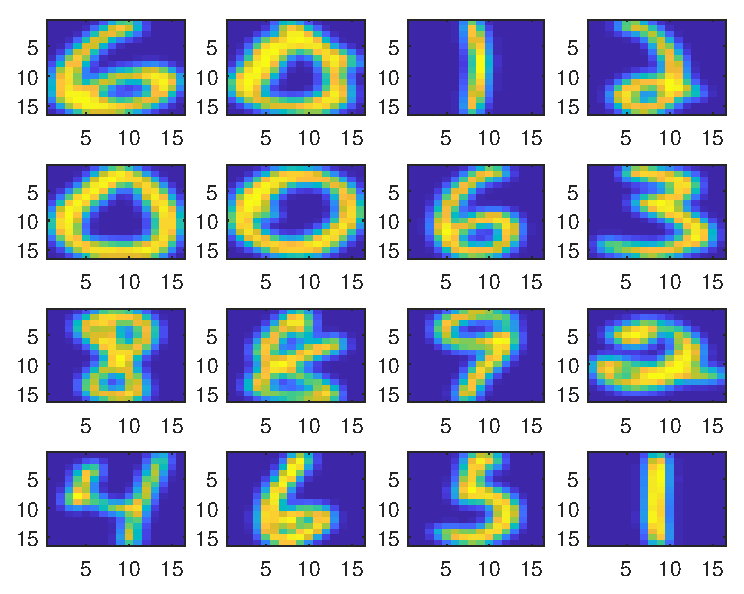
\includegraphics[scale=0.9]{First16.eps}
   \begin{center}Figure 1: first 16 images in train\_patterns.\end{center}
\end{center}
\begin{large}Step 02\end{large}
\begin{center}
   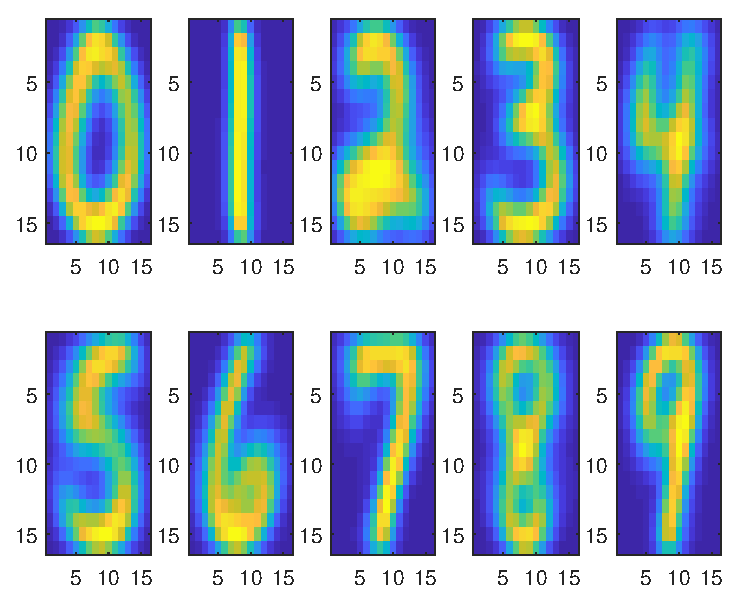
\includegraphics[scale=0.9]{10MDI.eps}
   \begin{center}Figure 2: The images of the mean of the 10 digits.\end{center}
\end{center}
\begin{flushright}Hangshi Jin \\913142686\end{flushright}
\begin{large}Step 03(c)\end{large}
   \[\text{test\_confusion}=\left[\begin{array}{cccccccccc} 656.0 & 1.0 & 3.0 & 4.0 & 10.0 & 19.0 & 73.0 & 2.0 & 17.0 & 1.0\\ 0 & 644.0 & 0 & 1.0 & 0 & 0 & 1.0 & 0 & 1.0 & 0\\ 14.0 & 4.0 & 362.0 & 13.0 & 25.0 & 5.0 & 4.0 & 9.0 & 18.0 & 0\\ 1.0 & 3.0 & 4.0 & 368.0 & 1.0 & 17.0 & 0 & 3.0 & 14.0 & 7.0\\ 3.0 & 16.0 & 6.0 & 0 & 363.0 & 1.0 & 8.0 & 1.0 & 5.0 & 40.0\\ 13.0 & 3.0 & 3.0 & 20.0 & 14.0 & 271.0 & 9.0 & 0 & 16.0 & 6.0\\ 23.0 & 11.0 & 13.0 & 0 & 9.0 & 3.0 & 354.0 & 0 & 1.0 & 0\\ 0 & 5.0 & 1.0 & 0 & 7.0 & 1.0 & 0 & 351.0 & 3.0 & 34.0\\ 9.0 & 19.0 & 5.0 & 12.0 & 6.0 & 6.0 & 0 & 1.0 & 253.0 & 20.0\\ 1.0 & 15.0 & 0 & 1.0 & 39.0 & 2.0 & 0 & 24.0 & 3.0 & 314.0 \end{array}\right]\]
\begin{large}Step 04(d)\end{large}
    \[\text{test\_svd17\_confusion}=\left[\begin{array}{cccccccccc} 772.0 & 2.0 & 1.0 & 3.0 & 1.0 & 1.0 & 2.0 & 1.0 & 3.0 & 0\\ 0 & 646.0 & 0 & 0 & 0 & 0 & 0 & 0 & 0 & 1.0\\ 3.0 & 6.0 & 431.0 & 6.0 & 0 & 3.0 & 1.0 & 2.0 & 2.0 & 0\\ 1.0 & 1.0 & 4.0 & 401.0 & 0 & 7.0 & 0 & 0 & 4.0 & 0\\ 2.0 & 8.0 & 1.0 & 0 & 424.0 & 1.0 & 1.0 & 5.0 & 0 & 1.0\\ 2.0 & 0 & 0 & 5.0 & 2.0 & 335.0 & 7.0 & 1.0 & 1.0 & 2.0\\ 6.0 & 4.0 & 0 & 0 & 2.0 & 3.0 & 399.0 & 0 & 0 & 0\\ 0 & 2.0 & 0 & 0 & 2.0 & 0 & 0 & 387.0 & 0 & 11.0\\ 2.0 & 9.0 & 1.0 & 5.0 & 1.0 & 1.0 & 0 & 0 & 309.0 & 3.0\\ 0 & 5.0 & 0 & 1.0 & 0 & 0 & 0 & 4.0 & 1.0 & 388.0 \end{array}\right]\]
\begin{large}Step 05(a)\end{large}
\\\\Both train\_patterns and test\_patterns store each digit as a column vector of 256$\times$1. In other word, each column vector contains all the entries of the 16$\times$16 gray image of one digit, in a way of stacking all the 16$\times$1 vectors into 256$\times$1 vector. Here the dataset is cut into 50/50 for training and testing. The training data is used to build the model within an algorithm to classify the true digit values of handwritten digits from 0 to 9, whereas the testing data is used to test the accuracy of the classification of the model within the algorithm used.
\\\\\begin{large}Step 05(b)\end{large}
\\\\In Step 02, train\_labels is used to gather all the images of the digits, and to sort them into the kind each of them truely belongs to. Then we sum up all the 256$\times$1 vectors of each kind of digit, and divide each of the sums by the size of corresponding kind of digit. The images of the mean of these 10 digits indicate that these 10 digits are well presented, which means it is reasonable to believe that the model can classify well-written digits easily within an algorithm.
\\\\\begin{large}Step 05(c)\end{large}
\\\\The simplest classification:
    \[\begin{array}{|c|c|c|c|c|c|c|c|c|c|} \hline0&1&2&3&4&5&6&7&8&9\\\hline91.11 & 89.32 & 91.18 & 87.83 & 76.58 & 83.38 & 78.84 & 89.77 & 76.44 & 74.41\\\hline \end{array}\]
SVD:\[\begin{array}{|c|c|c|c|c|c|c|c|c|c|}  \hline0&1&2&3&4&5&6&7&8&9\\\hline97.97 & 94.58 & 98.4 & 95.25 & 98.15 & 95.44 & 97.32 & 96.75 & 96.56 & 95.57\\\hline \end{array}\]
\begin{flushright}Hangshi Jin \\913142686\end{flushright}
Through the tables above, it is clear that 9 is the most difficult digit for Euclidean distance algorithm, and 1 for SVD algorithm; 2 is the easiest for both Euclidean distance and SVD algorithm. Instead of using the mean digit images as the simplest classification algorithm does, SVD has the advantage of gathering the variations of one kind digit images within the training dataset, using an orthogonal basis with rank 17. According to Professor Saito's lecutre, at rank 17, this algorithm performs the highest accuracy on classificaition of digit images. With this advantage, even if a digit image has large Euclidean distance from the mean digit image (bad handwritten), it can probably still be classified correctly because of the existence of the variation ranges of that kind digit image.
\\\\\begin{large}Step 05(d)\end{large}
\\\\From the tables above, it is clear to see that SVD has better performance on the results. Every kind digit classification by SVD hits over 90\% accuracy. This is because SVD is able to create a rank 17 approximation for every single digit image, which largely preserves the quality of the information of each digit image. In other words, in SVD, every single digit image is compared by its own approximation, not the mean digit image that is used by the simplest classification algorithm which can cause large Euclidean distances (approximation errors).
\end{document}